\documentclass{article}
\usepackage{graphicx} % Required for inserting images
\usepackage{float}

\title{2D Gray-Scott Model MPI}
\author{Skupina 16: Luka Pantar, Mark Loboda}
\date{April 2025}

\begin{document}

\maketitle

\section{Introduction}
\subsection{Serial}
This algorithm performs a reaction-diffusion system called the \textit{Gray-Scott model} that simulates the behavior of two species over time and space in two dimensions. Interesting patterns emerge from the simulation over time. The algorithm is using Finite Differ-
ences method and runs on one thread without any parallelization. For timing method, we used \textit{MPI\_Wtime} function to ensure any timing overhead is the same across the all experiments.

\subsection{Parallel}
This algorithm performs the same simulation but is run on a Distributed Memory System using MPI. We parallelized computation of grid rows, or rather strips. This involves distributing the work and exchanging data (to and bottom rows) between cooperating processes to update the grid values. Between each point in time, the grid pointers are swapped around to not require any copies between steps.

\section{Results}
We ran a benchmark of our algorithms where we ran each algorithm eight times for five different grid sizes (256, 512, 1024, 2048, 4096). The number of processes ranged between 1 and 64 in order to compare how the distribution speeds up the algorithm execution. We also discarded three of the worst times, as the times in some cases are too low to run consistently and sometimes resulted in much higher times, which could’ve been for other reasons and not the algorithm implementation itself. The resulting grid animation always stayed consistent, indicating correct working of the algorithm.


The figure ~\ref{fig:avg_times} shows that dividing the work to different processes is highly beneficial to execution time. We can observe that even parallel execution with one process in a little bit faster than serial algorithm. The reason most likely lies in different approach to indexing of the grid, as a flattened array is faster than a grid with x and y indexes.
Speedups were detected across the different grid sizes, as shown in figure ~\ref{fig:speedups}. The biggest gains were for grid size of 1024. There was a slight anomaly with 32 processes on grid size 256, which can be probably attributed to issues on the server. Larger grid size showed a small drop in speedup, but the execution times were still around thirty times faster for the 64 processes.

\begin{table}[H]
    \centering
    \begin{tabular}{| l | c || c | c | c | c | c |}
        \hline
        Algorithm & Processes & 256x256 & 512x512 & 1024x1024 & 2048x2048 & 4096x4096 \\
        \hline
        Serial & 1 & 12.24 & 37.74 & 203.31 & 550.16 & 1694.08 \\
        Parallel & 1 & 6.87 & 25.34 & 103.69 & 381.64 & 1319.38 \\
        Parallel& 2 & 3.79 & 12.93 & 40.34 & 175.09 & 804.93 \\
        Parallel& 4 & 2.92 & 6.67 & 23.66 & 116.34 & 431.43 \\
        Parallel& 16 & 1.05 & 3.51 & 10.68 & 45.16 & 163.33 \\
        Parallel& 32 & 6.87 & 2.34 & 6.38 & 24.29 & 94.10 \\
        Parallel& 64 & 0.97 & 1.65 & 4.27 & 13.23 & 50.04 \\
        \hline
    \end{tabular}
    \caption{Average total time per grid size for each algorithm and number of processes, measured in \textbf{milliseconds [ms]}.}
    \label{tbl:avg_times}
\end{table}


\begin{figure}[H]
    \centering
    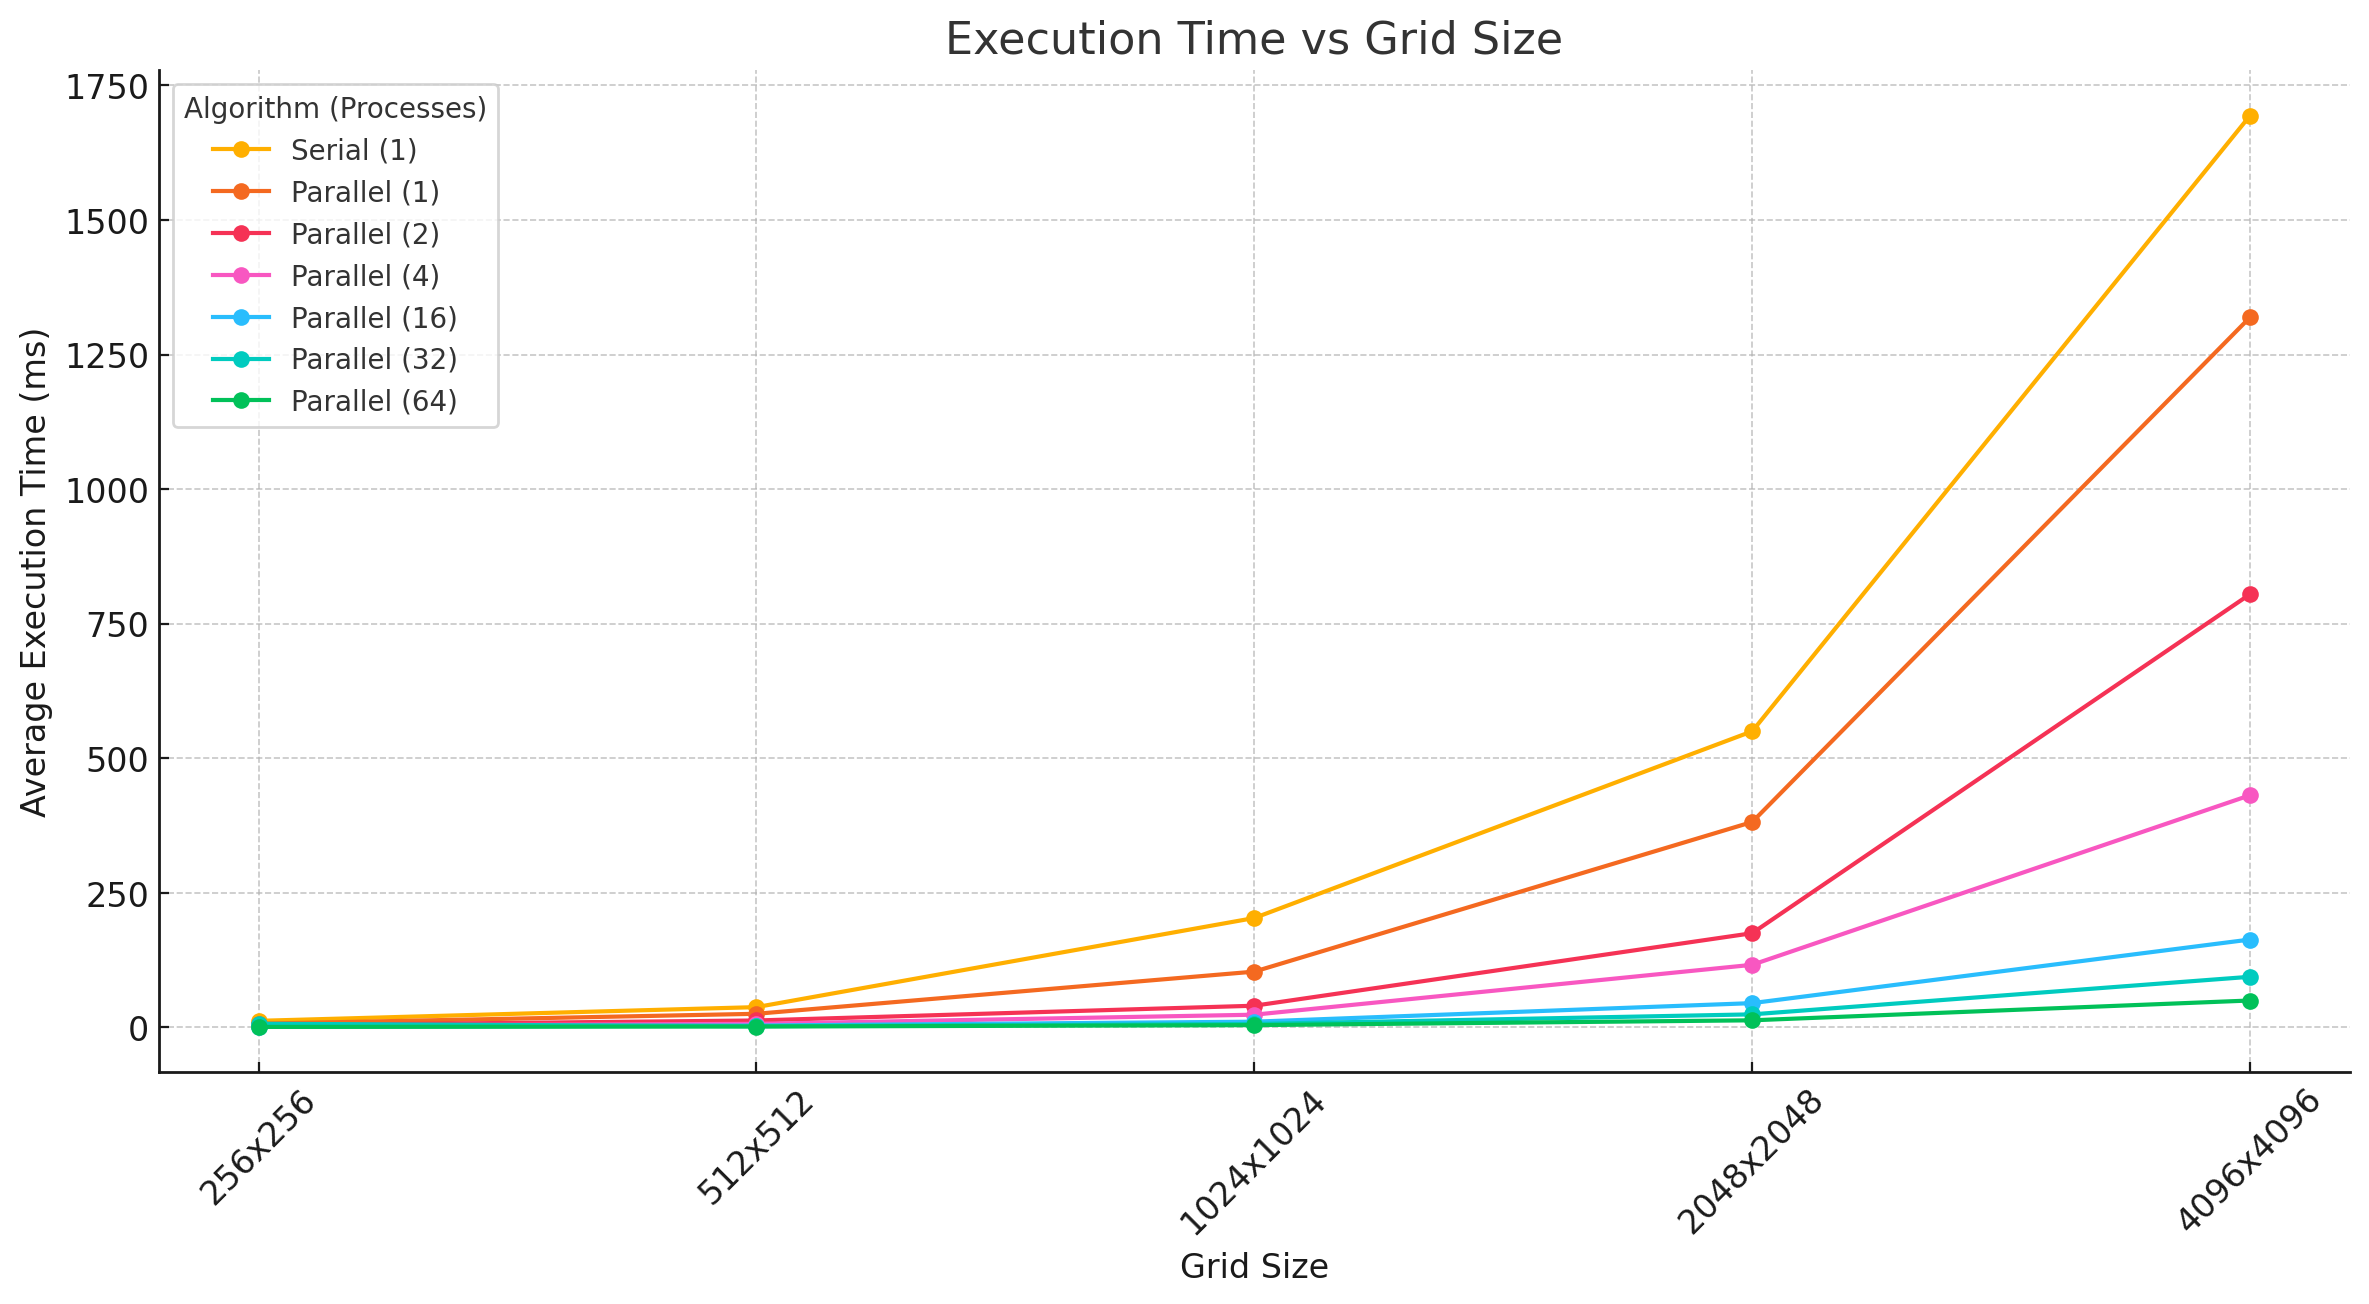
\includegraphics[width=1.1\linewidth]{img/graph1.png}
    \caption{Average execution time measured in \textbf{milliseconds [ms] in log scale} of each algorithm for each grid size, shown in Table~\ref{tbl:avg_times}.}
    \label{fig:avg_times}
\end{figure}


\begin{table}[H]
    \centering
    \begin{tabular}{| l || c | c | c | c | c |}
        \hline
        Processes & 256x256 & 512x512 & 1024x1024 & 2048x2048 & 4096x4096 \\
        \hline
1    &   1.78  & 1.49  & 1.96   &1.44&   1.28\\
2       &    3.23  & 2.92&  5.04 &  3.14  & 2.10\\
4       &    4.19  & 5.66 &  8.59 &  4.73  & 3.93\\
16     &    11.66&  10.75 & 19.03  &12.18 & 10.37\\
32      &    1.78 & 16.13 & 31.86 & 22.65 & 18.00\\
64      &   12.62 & 22.87 & 47.61 & 41.59 & 33.85\\
        \hline
    \end{tabular}
    \caption{Average speedup of parallel algorithm, calculated between execution times for each grid size and number of processes.}
    \label{tbl:speedups}
\end{table}

\begin{figure}[H]
    \centering
    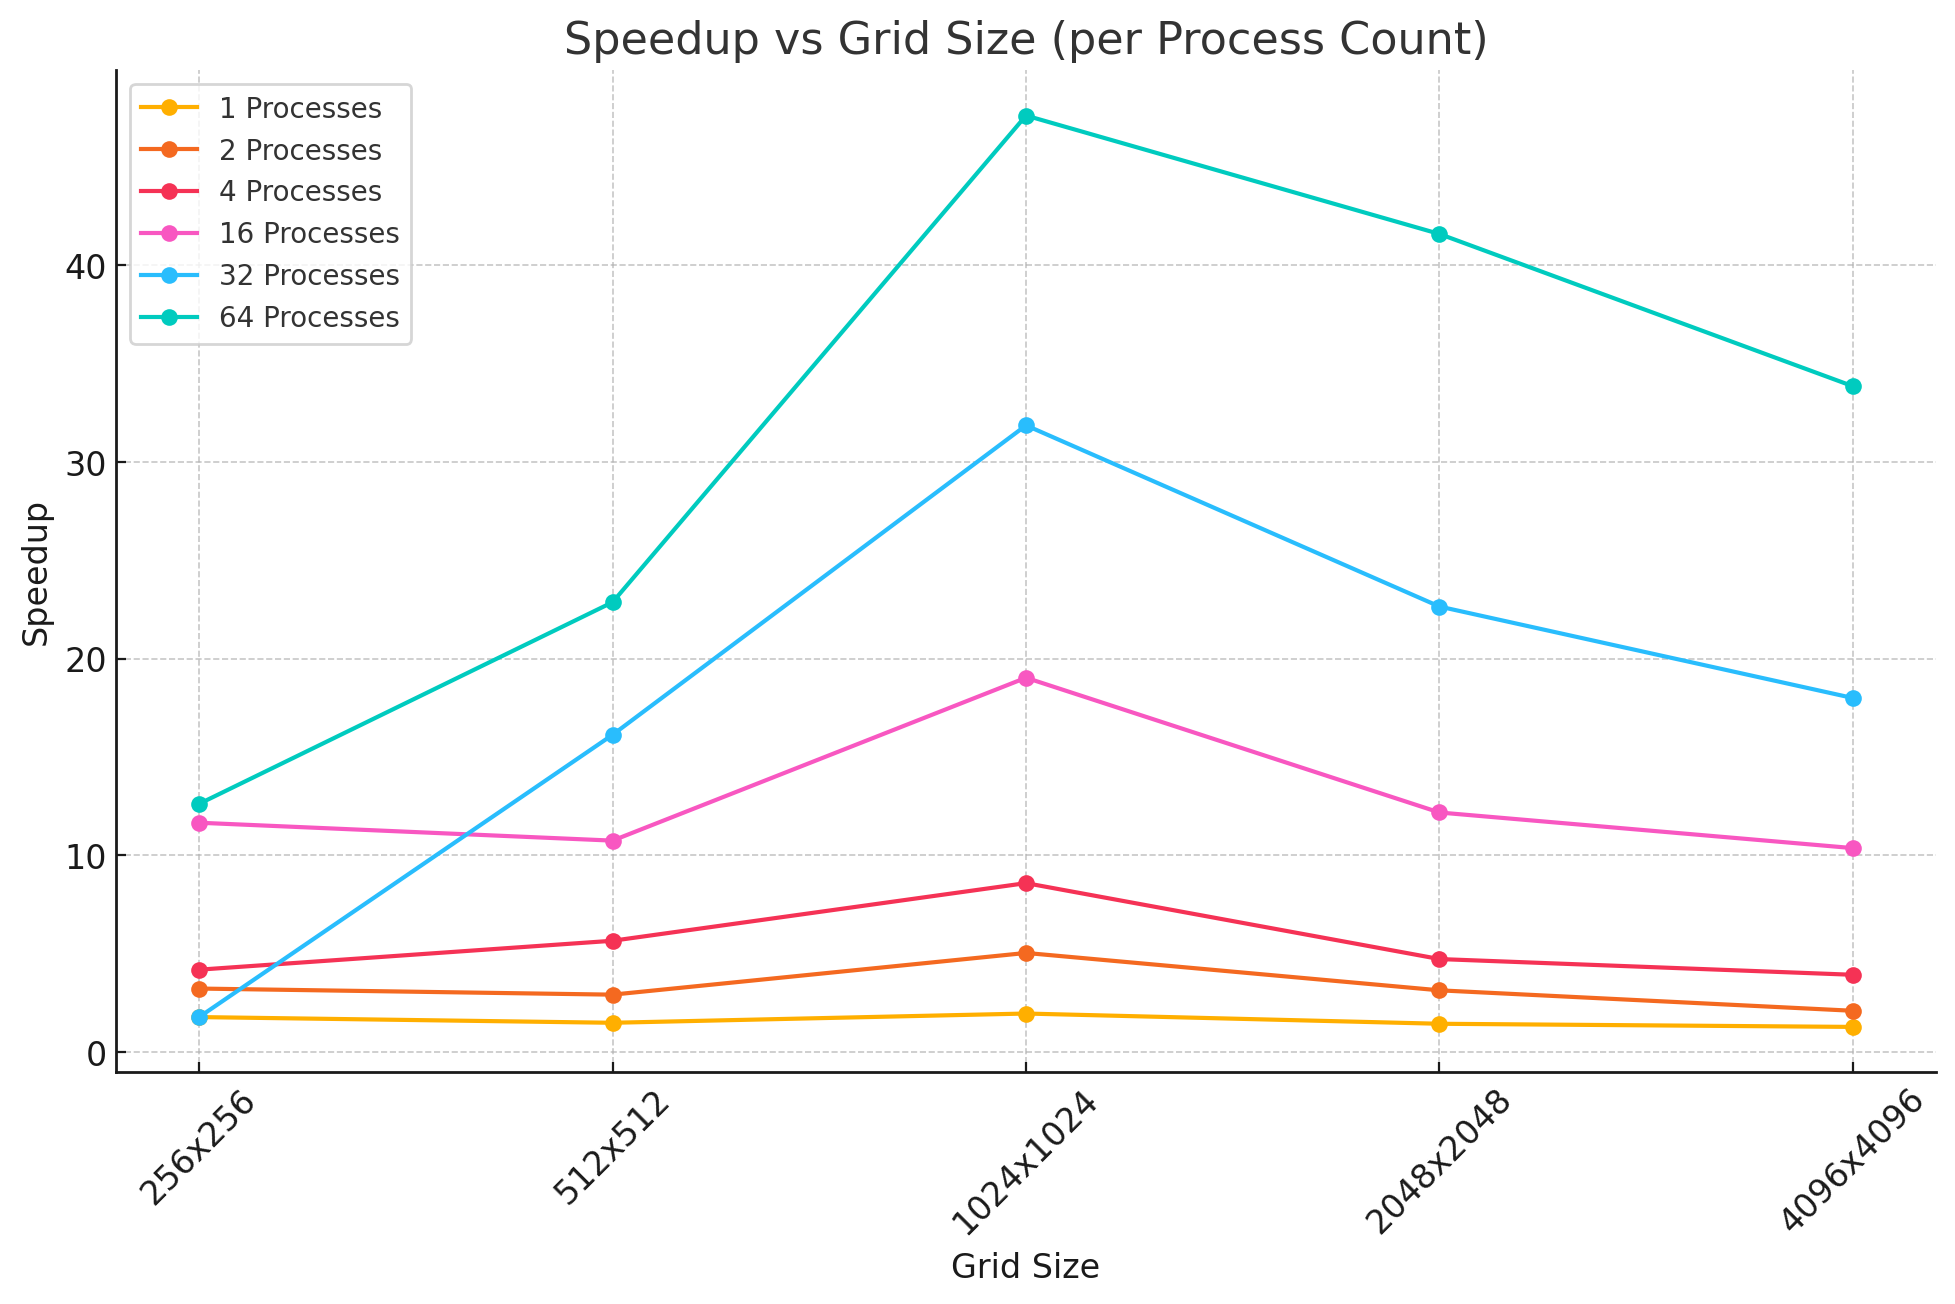
\includegraphics[width=1.0\linewidth]{img/graph2.png}
    \caption{Average speedup calculated between execution times for each grid size and number of processes, shown in Table~\ref{tbl:speedups}.}
    \label{fig:speedups}
\end{figure}

\end{document}
